\section{Tests of Parameters Performance}
%\begin{enumerate}
%\item Introduction to the section. What do we want and why. First we want to test A and the X. At last we want to test the complete system.
%\item Introduce how we will compare the tests and how we measure the quality -- Mean Squared Error (MSE).
%\item Subsection with the error measure
%\item Subsection with a introduction to the data sets -- AR and Toy Example data sets.
%\item Subsection with the performing of tests
%	\begin{itemize}
%	\item Talk about the choice for a initial A in the Cov-DL when D is under-complete. Random uniform distribution? or a Gaussian distribution. Show the errors of the real A and estimated A.
%	\item With the choice for A we now tests the choice for the number of segmentation in Cov-DL.
%	\item Test X with the found A. Make a comparison of the error for X and A in one plot.
%	\end{itemize}
%\end{enumerate}
With the implemented algorithms -- Cov-DL and M-SBL -- the goal is now to investigate the performance of each algorithm. The performance will be measure by a error measure -- the mean square error (MSE) -- this will be presented in the next section. To make a realistic conclusion on the performance values achieved from the MSE the performance of the algorithms will be compared to the MSE value of the performance of the algorithm with a known mixing matrix $\mathbf{A}$. All the tests will be done one the estimated matrices but for the comparison of these error measurement the true mixing matrix will be used. As the true $\mathbf{A}$ is used we can not compared the performance of Cov-DL but only M-SBL as this used the mixing matrix $\mathbf{A}$ as inputs. The Cov-DL algorithm will instead be tested for different choice of parameters, the initial $\mathbf{A}_{\text{ini}}$ using in the Cov-DL for the optimisation part of finding the matrix $\mathbf{D}$, and the segmentations in Cov-DL as well.
Each test will be looking at one parameter of the algorithm where it is the performance of that parameter there will be measured.

First at all, we will run a test, with random setting, to see how the error margin is for both algorithms.

\subsection{Error}
To evaluate performance of the algorithms we will be looking at the differences between the real and estimated matrices, mixing matrix $\mathbf{A}$ and source matrix $\mathbf{X}$.
For this task a mean squared error (MSE) method has been chosen. 
The MSE method measure the average squared difference between some estimated value and the actual value. 
%The MSE has the property of always being positive because of the randomness introduced in the method.
The MSE can be written as
\begin{align*}
\text{MSE} = \frac{1}{T} \sum_{i=1}^T (G_i - \hat{G}_i)^2,  
\end{align*}
with $T = \{M, k\}$ the numbers of rows of $\mathbf{A}$ or $\mathbf{X}$, $G_i = \{ \mathbf{A}_i, \mathbf{X}_i\}$ is a measurement row of the actual matrix and $\hat{G}_i = \{\hat{\mathbf{A}}_i,\hat{\mathbf{X}}_i\}$ is an estimated row of the estimated matrix.
The MSE is viewed as a measure of the quality of an estimator, in this case of how M-SBL and Cov-DL perform. 
For a large MSE value the estimated matrix/values are dispersed widely around its mean while for a small MSE value the estimated matrix/values is closely dispersed around the mean. 
Usually, a small MSE value indicate a good estimator but the value cannot be to small as this would indicate that the data has been overfitted \todo{Vi skal lige finde en god kilde som siger dette}. 
Therefore, a good MSE and therefore a good performance would be depending on how the data is scattered as widely scattered data may lead to a MSE value not close to zero but it would still be the a good measure for the estimator.

\subsection{Simulation of Data Sets}
For the test of the performance of the algorithms some simulated data sets will be used as we then know the real mixing matrix and source matrix which will be using when measuring the performance with MSE.

Two data sets has been made, one which is just a simple data set with simple measurement, and one which is more random and fluctuated -- more like real EEG measurements.

\subsubsection{Simple Data Set}
The simple data set is a date set which do not represent realistic data, EEG measurements, but is only used to confirm that the two algorithm works and to test the performance.
The simple data set is constructed from four different signals representing the sources of the source matrix $\mathbf{X}$: 
\begin{itemize}
\item[-] a sinus signal $\sin(2t)$
\item[-] a sinus signal $\sin(4t)$
\item[-] a sawtooth signal with period $2 \pi t$
\item[-] a sign signal of $\sin(3t)$
\end{itemize}
with $t$ being a time index defined in the interval $[0,10]$ with $L$ samples. Each of the four signal are randomly drawn and used to construct a source matrix $\mathbf{X}$ of size $k \times L$. Therefore some of the signals may occur two or more time as sources.
The mixing matrix $\mathbf{A}$ of size $M \times k$ is randomly generated from a Gaussian distribution. Its rows are then normalised. 
By multiplying the source matrix and the mixing matrix the measurement matrix $\mathbf{Y}$ is achieved.
The simple data set then consist of $\{ \mathbf{Y}, \mathbf{X}, \mathbf{A} \}$ which are the true values of the MMV model.

An illustration of the measurement matrix $\mathbf{Y}$ from the simple data set can be seen in figure \ref{fig:mix}. The data set is constructed for $M = 3$, $k = 4$ and $L = 1000$.
\begin{figure}[H]
\centering
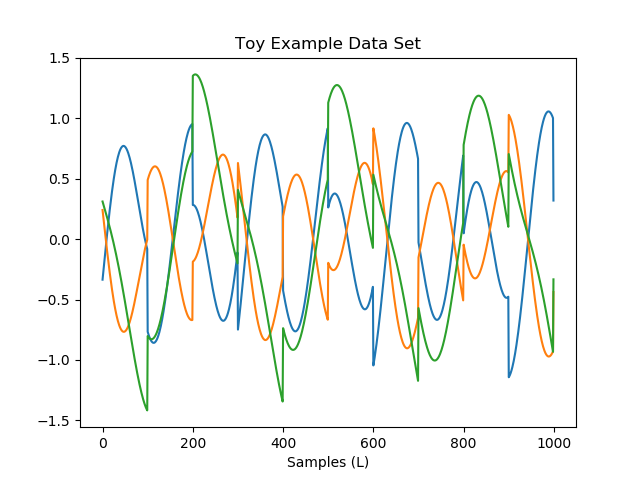
\includegraphics[scale=0.5]{figures/chapter6/Mix_Data_m3_n4_k4_L1000.png}
\label{fig:mix}
\caption{All the signal of the simple data set for $M = 3$, $k=4$ and $L=1000$.}
\end{figure}
\noindent

\subsubsection{Autoregressive Data Set}
The second data set illustrate a more realistic data set.
The data set is constructed from four different autoregressive processes representing the sources of the source matrix $\mathbf{X}$ \todo{Skal lige finde en god måde at skrive dem ind på}: 
\begin{itemize}
\item[-] $\mathbf{x}^{t} = \mathbf{a1}^{t-1} \cdot \mathbf{x}^{t-1} + \mathbf{a1}^{t-2} \cdot \mathbf{x}^{t-2} + \mathbf{w1}_t$
\item[-] $\mathbf{x}^{t+1} = \mathbf{a2}_t \cdot \mathbf{x}_{t-1} + \mathbf{a}_t \cdot \mathbf{x}_t + \mathbf{w}_t$
\item[-] $\mathbf{x}_{t+1} = \mathbf{a}_t \cdot \mathbf{x}_{t-2} + \mathbf{a}_t \cdot \mathbf{x}_t + + \mathbf{a}_t \cdot \mathbf{x}_{t-1} \mathbf{w}_t$
\item[-] $\mathbf{x}_{t+1} = \mathbf{a}_t \cdot \mathbf{x}_t + \mathbf{a}_t \cdot \mathbf{x}_{t-3} + \mathbf{w}_t$
\end{itemize}
Each of the four autoregressive processes are randomly drawn and used to construct a source matrix $\mathbf{X}$ of size $k \times L$. 
The mixing matrix $\mathbf{A}$ of size $M \times k$ is randomly generated as the same way as the mixing matrix from  the simple data set, from a Gaussian distribution and with its rows normalised. 
By multiplying the source matrix and the mixing matrix the measurement matrix $\mathbf{Y}$ is achieved.
The autoregressive data set then consist of $\{ \mathbf{Y}, \mathbf{X}, \mathbf{A} \}$ which are the true values of the MMV model.

An illustration of the autoregressive data set can be seen in figure \ref{fig:AR}. The data set is constructed for $M = 3$, $k = 4$ and $L = 1000$.
\begin{figure}[H]
\centering
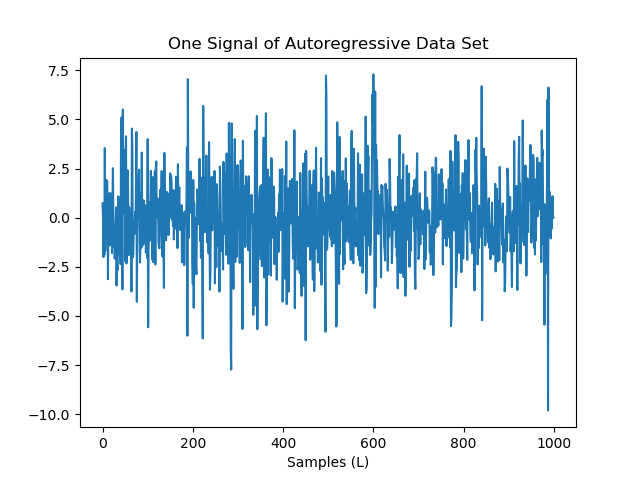
\includegraphics[scale=0.5]{figures/chapter6/AR_Data_m3_n4_k4_L1000.png}
\label{fig:AR}
\caption{All the signal of the toy example data set for $M = 3$, $k=4$ and $L=1000$.}
\end{figure}
\noindent

\subsection{Tests}
Before any testing of the performance of the algorithms one must test if the algorithm works. The Cov-DL and M-SBL has been tested with the simple data to see if the algorithms give us a results and how the performance of M-SBL differs when using an estimated mixing matrix and the true mixing matrix.

In the following figure we see the recovered sources aligned with the real source of a system with $M = 3$ and $k = 4$ for $L = 100$ -- a small system.
\begin{figure}[H]
\centering
    \begin{minipage}[t]{.45\textwidth}
        \centering
        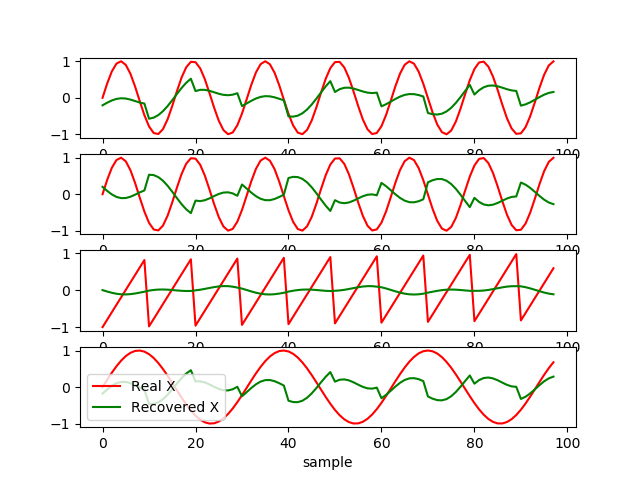
\includegraphics[scale=0.5]{figures/chapter6/test_of_algo_mix_data.png}
\label{fig:test_toy}
\caption{The $k$ recovered sources from M-SBL with the estimated mixing matrix $\mathbf{A}$}
    \end{minipage} 
    \hfill
    \begin{minipage}[t]{.45\textwidth}
        \centering
        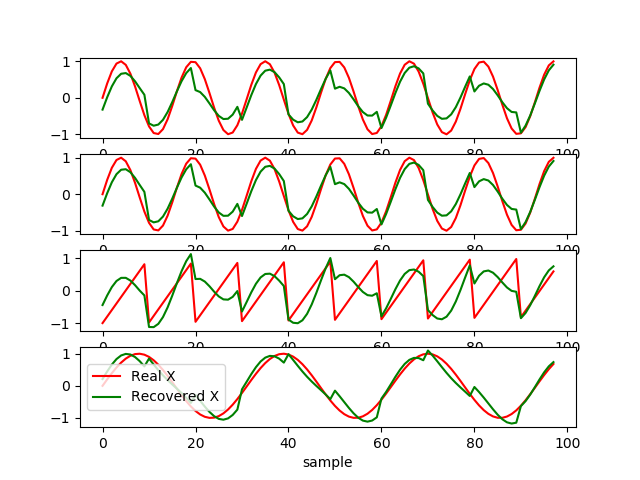
\includegraphics[scale=0.5]{figures/chapter6/test_of_algo_mix_data_realA.png}
\label{fig:test_toy_realA}
\caption{The $k$ recovered sources from M-SBL with the real mixing matrix $\mathbf{A}$}
    \end{minipage}
\end{figure}
\noindent
Furthermore, if we look at the at the mse then we have a representation error of

\begin{table}[H]
\centering
\begin{tabular}{|c|c|c|}
\hline
         & Estimated A & Real A \\ \hline
MSE of A & 1.76 & $\times$ \\ 
\hline 
MSE of X & 4.28 & 0.14 \\ 
\hline
\end{tabular} 
\caption{Toy Example Data Set}
\end{table}

\subsubsection{Initial A in Cov-DL}
In the Cov-DL algorithm described in XX the over-determined system use the principal component analysis to make an optimization problem from which the matrix $\mathbf{D}$ can be found. To solve the optimization problem and finding $\mathbf{D}$ an initial $\mathbf{A}_{\text{ini}}$ is used as a starting point in the optimization process. The choice of this initial $\mathbf{A}_{\text{ini}}$ will effect how the good an estimate our found mixing matrix $\hat{\mathbf{A}}$ is.

In this section we will be testing three different choice for $\mathbf{A}_{\text{ini}}$:
\begin{itemize}
\item[-] A matrix $\mathbf{A1}$ drawn from a continuous uniform distribution in the half-open interval $[0.0, 1.0)$
\item[-] A matrix $\mathbf{A2}$ drawn from a uniform distribution in the half-open interval $[-1.0, 1.0)$
\item[-] A matrix $\mathbf{A3}$ drawn from a Gaussian distribution with mean 0 and variance 1
\end{itemize}
The test of different initial A's will be performed on the AR data set as this resemble the real data, EEG measurements, at most. The goal with this test is to find the best initial A, with lowest error, such that when the baseline algorithm is used on realistic data, the parameters as been chosen with the best performance in mind -- leading to the best scenario of finding the true mixing matrix and source matrix from EEG measurements.

As the initial A will be used in finding an estimate for the mixing matrix which then be use to finding an estimate of the source matrix, we will look at the performance/error of both Cov-DL and M-SBL to find the best choice in both algorithms.

For the Cov-DL and M-SBL algorithm we are looking at a system of size $M = 8$, $k = 16$ and $L = 1000$. Furthermore, for the Cov-DL the data has been divided in segments of 10 samples.

\begin{table}[H]
\centering
\begin{tabular}{|c|c|c|c|}
\hline 
 & $\mathbf{A1}$ & $\mathbf{A2}$ & $\mathbf{A3}$ \\ 
\hline 
MSE of A & 1.09 & 1.12 & 1.13 \\ 
\hline 
MSE of X & 0.72 & 0.74 & 0.72 \\ 
\hline 
\end{tabular} 
\caption{Toy Example Data Set}
\end{table}
\noindent

\begin{table}[H]
\centering
\begin{tabular}{|c|c|c|c|}
\hline 
 & $\mathbf{A1}$ & $\mathbf{A2}$ & $\mathbf{A3}$ \\ 
\hline 
MSE of A & 2.04 & 2.14 & 1.99 \\ 
\hline 
MSE of X & 9.81 & 9.09 & 9.73 \\ 
\hline
\end{tabular} 
\caption{AR Data Set}
\end{table}

\begin{figure}[H]
\centering
    \begin{minipage}[t]{.45\textwidth}
        \centering
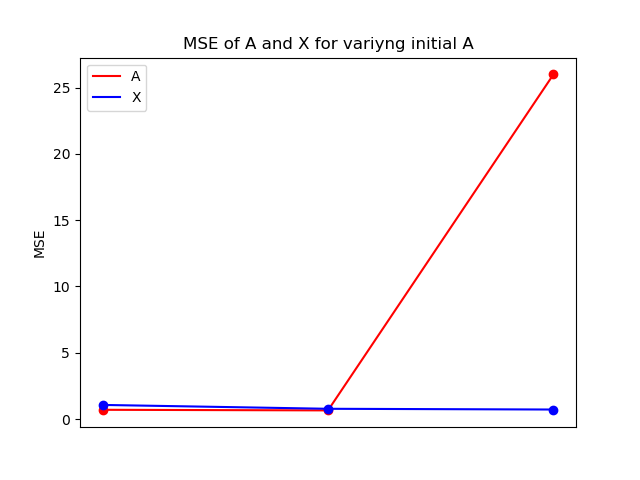
\includegraphics[scale=0.5]{figures/chapter6/Mix_Error_initial_A_m8_k16_L1000.png}
\label{fig:initialA_mix}
\caption{Toy Example Data Set}
    \end{minipage} 
    \hfill
    \begin{minipage}[t]{.45\textwidth}
        \centering
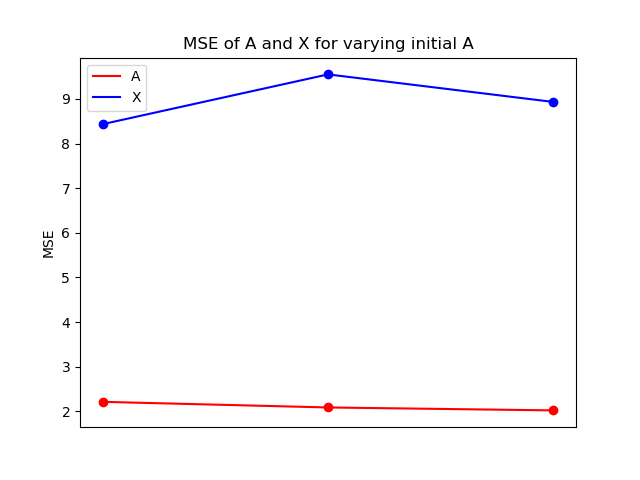
\includegraphics[scale=0.5]{figures/chapter6/AR_Error_initial_A_m8_k16_L1000.png}
\label{fig:initialA_AR}
\caption{AR Data Set}
    \end{minipage}
\end{figure}
\noindent


\subsubsection{Segmentation in Cov-DL}
\begin{figure}[H]
\centering
    \begin{minipage}[t]{.45\textwidth}
        \centering
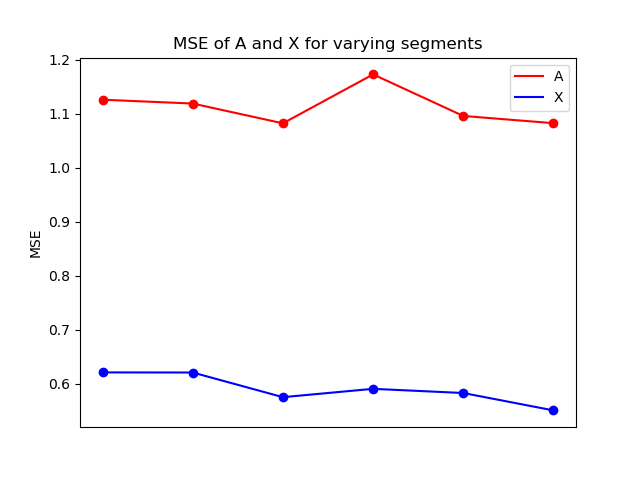
\includegraphics[scale=0.5]{figures/chapter6/Mix_Error_vary_covseg_m8_k16_L1000.png}
\label{fig:seg_mix}
\caption{Toy Example Data Set}
    \end{minipage} 
    \hfill
    \begin{minipage}[t]{.45\textwidth}
        \centering
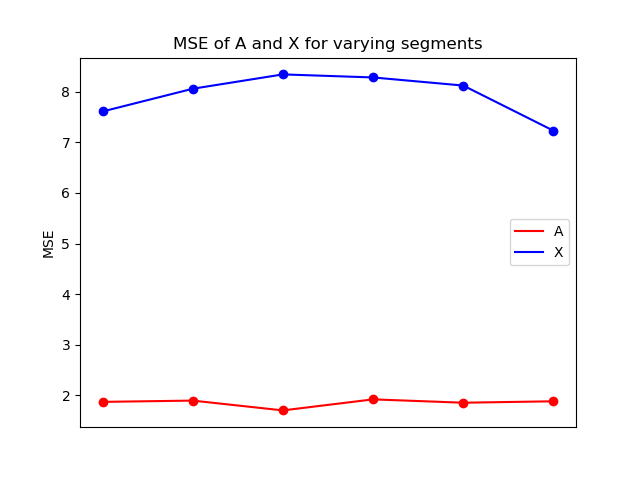
\includegraphics[scale=0.5]{figures/chapter6/AR_Error_vary_covseg_m8_k16_L1000.png}
\label{fig:seg_AR}
\caption{AR Data Set}
    \end{minipage}
\end{figure}
\noindent


\begin{table}[H]
\centering
\begin{tabular}{|c|c|c|c|c|c|c|}
\hline 
\textbf{Toy Example Data Set} & & & & & & \\ \hline
 & 10 & 20 & 30 & 40 & 50 & 60 \\ 
\hline 
MSE of A & 1.13 & 1.12 & 1.08 & 1.17 & 1.10 & 1.08 \\ 
\hline 
MSE of X & 0.62 & 0.62 & 0.58 & 0.59 & 0.58 & 0.55 \\ 
\hline
\\ \hline
\textbf{AR Data Set} & & & & & & \\ \hline
 & 10 & 20 & 30 & 40 & 50 & 60 \\ 
\hline 
MSE of A & 1.82 & 1.85 & 1.88 & 1.93 & 1.86 & 1.97 \\ 
\hline 
MSE of X & 10.76 & 9.98 & 10.23 & 11.33 & 9.85 & 10.10 \\ 
\hline
\end{tabular} 
\caption{Toy and AR Data Set}
\end{table}

